\documentclass[12pt]{article}
\usepackage{graphicx,import}
\usepackage{float}
\usepackage[svgnames]{xcolor} 
\usepackage{makecell}
\usepackage{fancyhdr}
\usepackage{subcaption}
\usepackage{hyperref}
\usepackage{enumitem}
\usepackage{cite}
\usepackage[many]{tcolorbox}
\usepackage{listings }
\usepackage[a4paper, total={6in, 8in} , bottom = 25mm , top = 25mm, headheight = 1.25cm , includehead,includefoot,heightrounded ]{geometry}
\usepackage{afterpage}
\usepackage{amssymb}
\usepackage{pdflscape}
\usepackage{gensymb}
\usepackage{textcomp}
\usepackage{tikz,pgfplots}
\usepackage{xecolor}
\usepackage{rotating}
\usepackage{pdfpages}
\usepackage[Kashida]{xepersian}
\usepackage[T1]{fontenc}
\usepackage{tikz}
\usepackage[utf8]{inputenc}
\usepackage{PTSerif} 
\usepackage{seqsplit}
\usepackage{hhline}
\usepackage{pgfgantt}
\usepackage{graphicx}
\usepackage{fontspec}

\graphicspath{ {./images/} }

\renewcommand\theadalign{bc}
\renewcommand\theadfont{\bfseries}
\renewcommand\theadgape{\Gape[4pt]}
\renewcommand\cellgape{\Gape[4pt]}

\usepackage[edges]{forest}

\usepackage{listings}
\usepackage{xcolor}

\hypersetup{
	colorlinks   = true, %Colours links instead of ugly boxes
	urlcolor     = blue, %Colour for external hyperlinks
	linkcolor    = blue, %Colour of internal links
	citecolor   = red %Colour of citations
}
 
\definecolor{codegreen}{rgb}{0,0.6,0}
\definecolor{codegray}{rgb}{0.5,0.5,0.5}
\definecolor{codepurple}{rgb}{0.58,0,0.82}
\definecolor{backcolour}{rgb}{0.95,0.95,0.92}
 
\NewDocumentCommand{\codeword}{v}{
\texttt{\textcolor{blue}{#1}}
}
\lstset{language=java,keywordstyle={\bfseries \color{blue}}}


\lstdefinestyle{mystyle}{
    backgroundcolor=\color{backcolour},   
    commentstyle=\color{codegreen},
    keywordstyle=\color{magenta},
    numberstyle=\tiny\color{codegray},
    stringstyle=\color{codepurple},
    basicstyle=\ttfamily\normalsize,
    breakatwhitespace=false,         
    breaklines=true,                 
    captionpos=b,                    
    keepspaces=true,                 
    numbers=left,                    
    numbersep=5pt,                  
    showspaces=false,                
    showstringspaces=false,
    showtabs=false,                  
    tabsize=2
}

\lstset{style=mystyle}

\setmainfont[Path = fonts/]{Bahij Nazanin-Regular}
\settextfont[Scale=1.2, Path = fonts/ ,BoldFont={Bahij Nazanin-Bold} , ItalicFont = {IRNazaninIranic}]{Bahij Nazanin-Regular}
% \setlatintextfont[Scale = 1.0]{Garamond}
% \DefaultMathsDigits 
\DeclareMathSizes{11}{19}{13}{9} 
%\DeclareMathSizes{12}{14.4}{8}{9}





\newenvironment{changemargin}[2]{%
\begin{list}{}{%
\setlength{\topsep}{0pt}%
\setlength{\leftmargin}{#1}%
\setlength{\rightmargin}{#2}%
\setlength{\listparindent}{\parindent}%
\setlength{\itemindent}{\parindent}%
\setlength{\parsep}{\parskip}%
}%
\item[]}{\end{list}}


\definecolor{foldercolor}{RGB}{124,166,198}

\tikzset{pics/folder/.style={code={%
    \node[inner sep=0pt, minimum size=#1](-foldericon){};
    \node[folder style, inner sep=0pt, minimum width=0.3*#1, minimum height=0.6*#1, above right, xshift=0.05*#1] at (-foldericon.west){};
    \node[folder style, inner sep=0pt, minimum size=#1] at (-foldericon.center){};}
    },
    pics/folder/.default={20pt},
    folder style/.style={draw=foldercolor!80!black,top color=foldercolor!40,bottom color=foldercolor}
}

\forestset{is file/.style={edge path'/.expanded={%
        ([xshift=\forestregister{folder indent}]!u.parent anchor) |- (.child anchor)},
        inner sep=1pt},
    this folder size/.style={edge path'/.expanded={%
        ([xshift=\forestregister{folder indent}]!u.parent anchor) |- (.child anchor) pic[solid]{folder=#1}}, inner xsep=0.6*#1},
    folder tree indent/.style={before computing xy={l=#1}},
    folder icons/.style={folder, this folder size=#1, folder tree indent=3*#1},
    folder icons/.default={12pt},
}

\begin{document}


%%% title pages
\begin{titlepage}
\begin{center}
        
\vspace*{0.7cm}


\includegraphics[width=0.4\textwidth]{sharif1.png}\\
\vspace{0.5cm}
\textbf{ \Huge{\emph ‌آزمایشگاه سخت‌افزار} }\\
\vspace{0.5cm}
\textbf{ \Large{ پروپوزال پروژه} }
\vspace{0.2cm}
       
 
      \large \textbf{دانشکده مهندسی کامپیوتر}\\\vspace{0.2cm}
    \large   دانشگاه صنعتی شریف\\\vspace{0.2cm}
       \large   ﻧﯿﻢ سال اول 02-01 \\\vspace{0.2cm}
      \noindent\rule[1ex]{\linewidth}{1pt}
استاد:\\
    \textbf{{جناب آقای دکتر اجلالی}}


دستیار آموزشی:\\
\textbf{{جناب آقای دکتر فصحتی}}

    \vspace{0.25cm}
    
    موضوع پروژه:\\
    
    \textbf{{دید در شب اتومبیل}}
    
    \vspace{0.35cm}
    
    
        شماره گروه:
    \textbf{{۶}}\\
    
اعضای گروه:\\

    \textbf{{علیرضا شاطری}}
    \\
   
    \textbf{{رضا امینی}}
\end{center}
\end{titlepage}
%%% title pages


%%% header of pages
\newpage
\pagestyle{fancy}
\fancyhf{}
\fancyfoot{}
\cfoot{\thepage}
\chead{}
\rhead{
\includegraphics[width=0.1\textwidth]{sharif.png}}
\lhead{پروپوزال پروژه}
%%% header of pages

\newfontfamily\terminal{Courier New Bold}

\KashidaOff
 \newcommand{\inlineLatin}[1]{
	\small{\lr{{\terminal #1}}}
}


\tableofcontents
\listoffigures
\listoftables

\newpage
\section{مقدمه}

هدف این پروژه ساخت سیستمی‌ست که با استفاده از تعدادی سنسور و چراغ، سعی دارد به کمک رانندگان اتومبیل بیاید. این سیستم به کمک یک ماژول دوربین تشخیص حرارت و با کمک روش‌های پردازش تصویر می‌تواند وجود یک موجود زنده یا عابر پیاده را زودتر از راننده در شب متوجه شود و به راننده هشدار دهد. همچنین چراغ‌های اتومبیل را به گونه‌ای تنظیم می‌کند تا به سمت آن موجود زنده نور را هدایت کند.



\begin{table}[H]
	\centering
	\begin{tabular}{|l|l|l|} 
		\hline
		\makecell{\textbf{ردیف}} & \makecell{\textbf{ویژگی}}                                         & \makecell{\textbf{توضیحات}}                                                                                         \\ 
		\hhline{|===|}
		۱             & \makecell{\textbf{تشخیص موجود زنده}}                               &
		\makecell{
		    از طریق یک دوربین حرارتی، بدن موجود 
		    \\ 
		    زنده را 
		    که دمایش با محیط اطراف
		    \\
		    متفاوت است تشخیص می‌دهد.
		 }           \\ 
		\hline
		۲             & \makecell{ \textbf{هشدار به راننده}    }                           & \makecell{
		پس از شناسایی موجود زنده باید او را
		\\
		از موجود زنده با خبر کند. این کار می‌تواند 
		\\
		از طریق روشن کردن یک چراغ خطر و یا
        \\  یک صدای اخطار 
		باشد.
		 }                   \\ 
		\hline
		
		۳             & \makecell{\textbf{هدایت نور اتومبیل}\\  \textbf{به سمت موجود زنده}}
		  &
		 \makecell{
		    چراغ‌های اتومبیل باید به سمت 
		    \\
		    موجود زنده هدایت شود تا \\
		    راننده نیز موجود زنده را ببیند.
		  }                                \\ 

		  		
		۴             & \makecell{\textbf{ذخیره تاریخچه}}
		  &
		 \makecell{
		    باید بتوان تاریخچه‌ی شناسایی 
		    \\
		    موجودات زنده را ذخیره کرد
		    \\
		     و در صورت نیاز به کاربر نشون داد.
		  }                                \\ 
		\hline
	\end{tabular}
\caption{\label{features}جدول ویژگی‌های اصلی محصول}
\end{table}



\newpage
\section{روش انجام پروژه}

\subsection{طرح کلی پروژه}

در این پروژه از برد رزپری پای ۳  استفاده خواهد شد. چراغ‌ها و سنسورهای محیطی به این برد متصل می شوند و از طریق رزبری اطلاعات آن ها پردازش و نتیجه توسط رزپری روی چراغ‌های LED نمایش داده می‌شود.
\\
\\
کد بخش نرم افزاری را با زبان Python و کتابخانه‌‌های مربوط به همین زبان پیاده‌سازی می‌کنیم. چراغ‌های LED نیز به برد وصل می‌شوند. همچنین از ماژول دوربین حرارتی آرایه‌ای \lr{AMG8833 IR 8x8} برای تصویربرداری حرارتی و پردازش دمایی محیط اطراف استفاده خواهیم کرد. همچنین زمان دقیق اخطار‌ها را درون فایلی در رزپری قرار می‌دهیم و در زمان نیاز می‌توان رزپری را به مانیتور متصل کرده و فایل را به نمایش در آورد. 


\subsection{ماژول‌ها}

\subsubsection{دوربین حرارتی}

یک آرایه سنسور مادون قرمز کم هزینه است که توسط پاناسونیک توسعه یافته است. برای استفاده با میکروکنترلرها در یک ماژول با شیفترهای سطح و تنظیم کننده ولتاژ یکپارچه شده است که برق و داده 3 تا 5 ولت را می دهد.
\\
این سنسور تنها 64 پیکسل (8×8) دارد که خیلی زیاد نیست اما برای آزمایش کافی و کار با آن ساده است، همچنین قیمت مناسبی نیز دارد. 
\\
ماژول را می‌توان به راحتی به برد متصل کرد و داده‌های دمایی تصویر را دریافت و پردازش نمود.


\begin{figure}[h]
	\begin{center}
		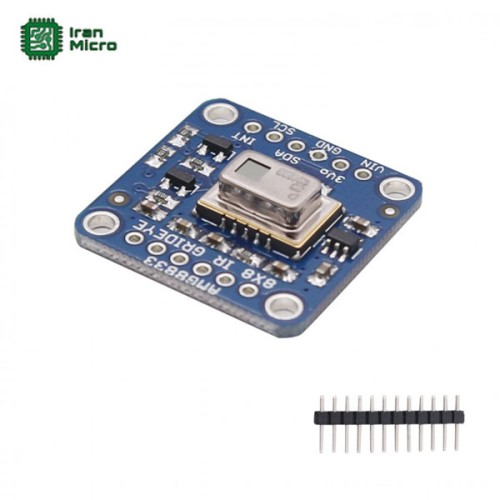
\includegraphics[width=0.5\textwidth]{AMG8833-module-1-500x500.jpg}
	\end{center}
	\caption{\lr{KY-015}}
\end{figure}


\subsubsection{رزپری ۳}

\begin{figure}[h]
	\begin{center}
		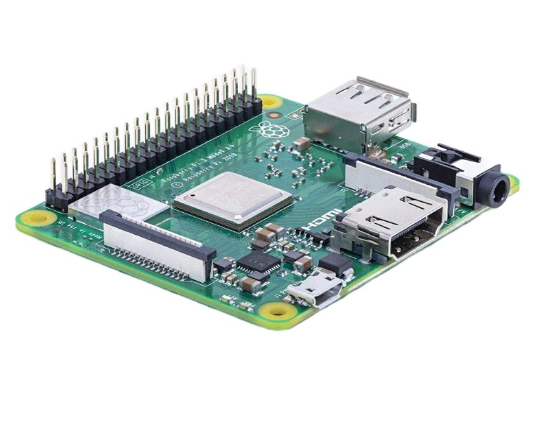
\includegraphics[width=0.5\textwidth]{raspberry.png}
	\end{center}
	\caption{\lr{AD8232}}
\end{figure}

تراشه پردازنده این محصول \lr{Broadcom BCM2837B0} و نوع پردازنده \lr{Cortex-A53 (ARMv8)} میباشد. مقدار رم ۴ گیگابایت است و فاقد حافظه ذخیره سازی داخلی میباشد. آداپتور مناسب این محصول 5 ولت و 2.5 آمپر میباشد. چون این برد حافظه داخلی ندارد، نیاز است تا یک حافظه خارجی مانند فلش به آن متصل نمود و داده‌هایی که نیاز به ثبت دائمی دارند را در آن ذخیره کرد.



\subsubsection{دوربین دید در شب (جایگزین دوربین حرارتی)}

\begin{figure}[h]
	\begin{center}
		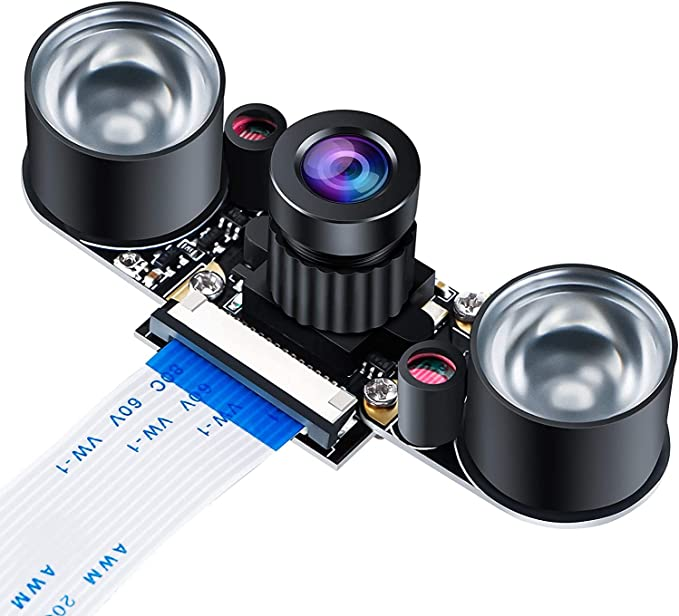
\includegraphics[width=0.5\textwidth]{camera.jpg}
	\end{center}
	\caption{\lr{MQ135}}
\end{figure}

دوربین دید در شب \lr{Raspberry Pi} ما مستقیماً به کانکتور\lr{ CSI Raspberry Pi} متصل می شود (برای استفاده با Pi Zero به آداپتور نیاز دارد) و دارای دو نورافکن LED مادون قرمز با شدت بالا برای ضبط در شب است! LED های IR مستقیماً از پورت CSI تغذیه می شوند و می توانند یک منطقه را تا فاصله 8 متری روشن کنند! در آزمایش، بهترین تصاویر در فاصله 3 تا 5 متری ثبت شد. این دوربین همچنین دارای لنز با فاصله کانونی 3.6 میلی متری قابل تنظیم و زاویه دید 75.7 درجه است.
\\
\\
این دوربین دید در شب \lr{Raspberry Pi} از همان \lr{OV5647} به عنوان دوربین استاندارد \lr{Raspberry Pi} استفاده می کند و بنابراین می تواند تصویری با وضوح 5 مگاپیکسل شفاف یا فیلمبرداری 1080p HD با سرعت 30 فریم بر ثانیه ارائه دهد!


\newpage
\subsection{سایر موارد}

در زیر جدول هزینه‌های تخمینی پروژه آورده شده است.



\begin{table}[h]
	\centering
	\begin{tabular}{|c|c|c|} 
		\hline
		\textbf{ردیف} & \textbf{قطعه}  &
		\makecell{
			\textbf{فی}\\
		 \textbf{ (هزارتومان)}
	}   \\ 
		\hhline{|===:b|}
		
		1             &
		\makecell{
		رزپری پای
		}
		  & \lr{3100} \\ 
		\hline
		2             & 
		\makecell{
		دوربین حرارتی
	}
		 & \lr{1100} \\ 
		\hline
				3             & 
		\makecell{
		USB
	}
		 & \lr{100} \\ 
		\hline
				4             & 
		\makecell{
		 LED & Board
	}
		 & \lr{50} \\ 
		\hline
		& \textbf{مجموع} &   \lr{4350}    \\
		\hline
	\end{tabular}
\caption{برآورد هزینه‌ها طراحی اول}
\end{table}

\begin{table}[h]
	\centering
	\begin{tabular}{|c|c|c|} 
		\hline
		\textbf{ردیف} & \textbf{قطعه}  &
		\makecell{
			\textbf{فی}\\
		 \textbf{ (هزارتومان)}
	}   \\ 
		\hhline{|===:b|}
		
		1             &
		\makecell{
		رزپری پای
		}
		  & \lr{3100} \\ 
		\hline
		2             & 
		\makecell{
		دوربین دید در شب
	}
		 & \lr{4000} \\ 
		\hline
				3             & 
		\makecell{
		USB
	}
		 & \lr{100} \\ 
		\hline
				4             & 
		\makecell{
		 LED & Board
	}
		 & \lr{50} \\ 
		\hline
		& \textbf{مجموع} &   \lr{7250}    \\
		\hline
	\end{tabular}
\caption{برآورد هزینه‌ها طراحی دوم}
\end{table}

\end{document}



